\section{Exercise 2.1}
Starting from the results of Experiment 4 of Assignment 1 the following approaches to improve the network performance were tested:\\
\begin{enumerate}[label=(\roman*)]
    \item use all available training data
    \item train for a longer time
    \item shuffle the order of the training set at the beginning of every epoch
\end{enumerate}
The results after Experiment 4 of Assignment 1
(lambda=0, n\_epochs=40, n\_batch=100, eta=0.1) were as follows:\\
training loss: 1.899\\
validation loss: 1.958\\
accuracy: 37.38\%\\

% \begin{table}[ht]
% \begin{tabular}{|l|l|l|l|l|}
% \hline
%                     & \textbf{Experiment 1} & \textbf{Experiment 2} & \textbf{Experiment 3} & \textbf{Experiment 4} \\ \hline
% \textbf{Training}   & 5.074                 & 1.609                 & 0.3908                & 1.899                 \\ \hline
% \textbf{Validation} & 7.526                 & 1.791                 & 1.903                 & 1.958                 \\ \hline
% \end{tabular}
% \caption{Summary of final loss}
% \label{tab:summary_loss}
% \end{table}

% \begin{table}[ht]
% \begin{tabular}{|l|l|l|l|l|}
% \hline
%                   & \textbf{Experiment 1} & \textbf{Experiment 2} & \textbf{Experiment 3} & \textbf{Experiment 4} \\ \hline
% \textbf{Accuracy} & 27.84\%               & 39.08\%               & 39.46\%               & 37.38\%               \\ \hline
% \end{tabular}
% \caption{Summary of final accuracy}
% \label{tab:summary_accuracy}
% \end{table}

\newpage

\subsection{Results Improvement (i)} 

final training loss 1.920\\
final validation loss 1.935\\
final accuracy 0.3786\\
    \begin{figure}[ht]
        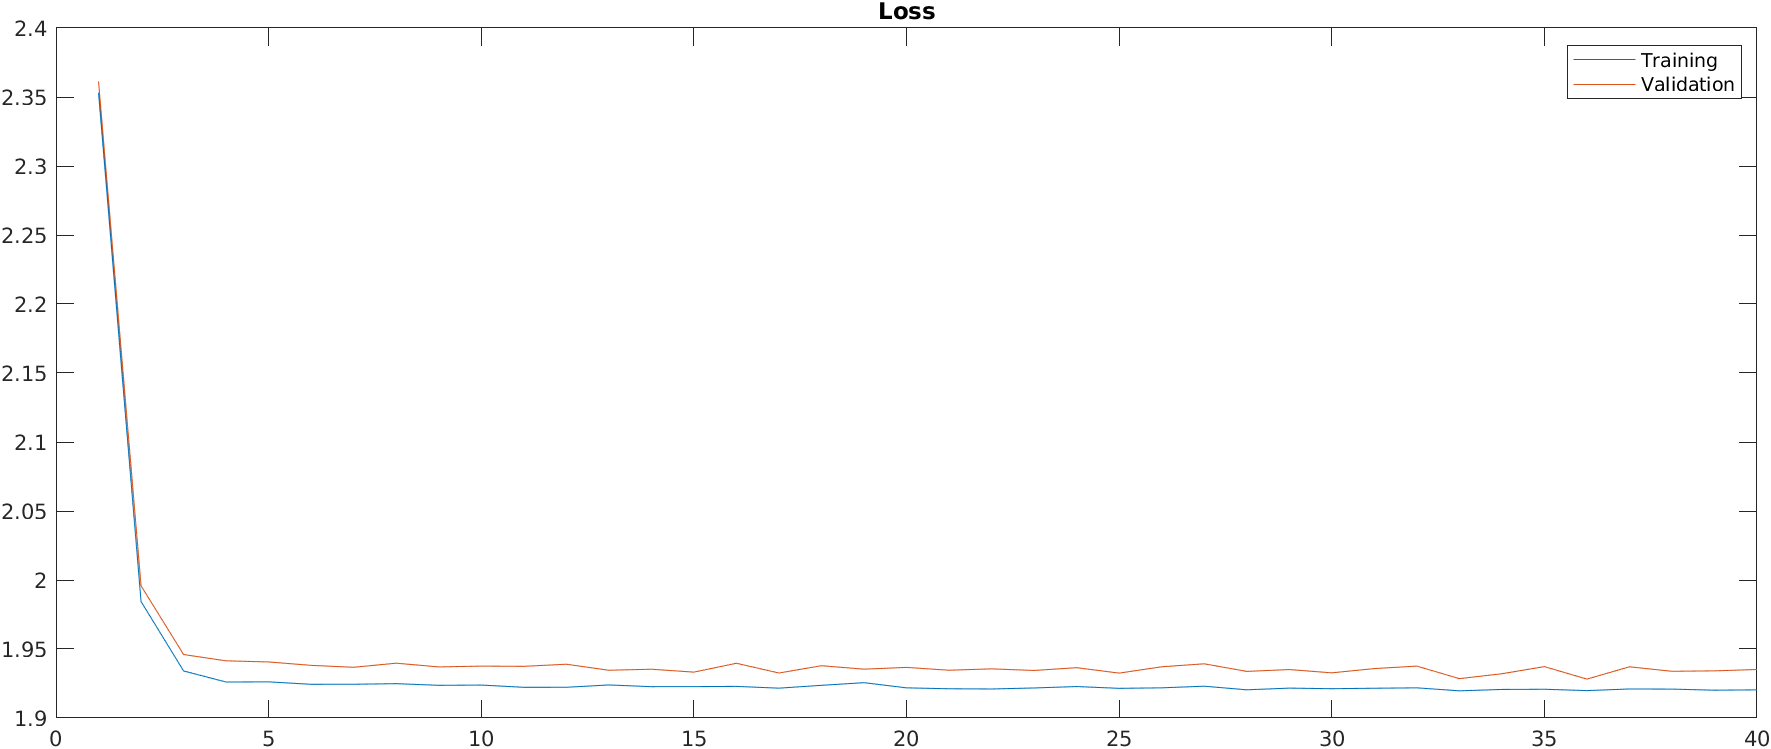
\includegraphics[width=\textwidth]{../code/result_pics/lambda=1, n_epochs=40, n_batch=100, eta=.001 all data for training/loss.png}
        \caption{Improvement (i) Loss (lambda=1, n\_epochs=40, n\_batch=100, eta=0.001)}
        \label{fig:lossa}
    \end{figure}
    \begin{figure}[ht]
        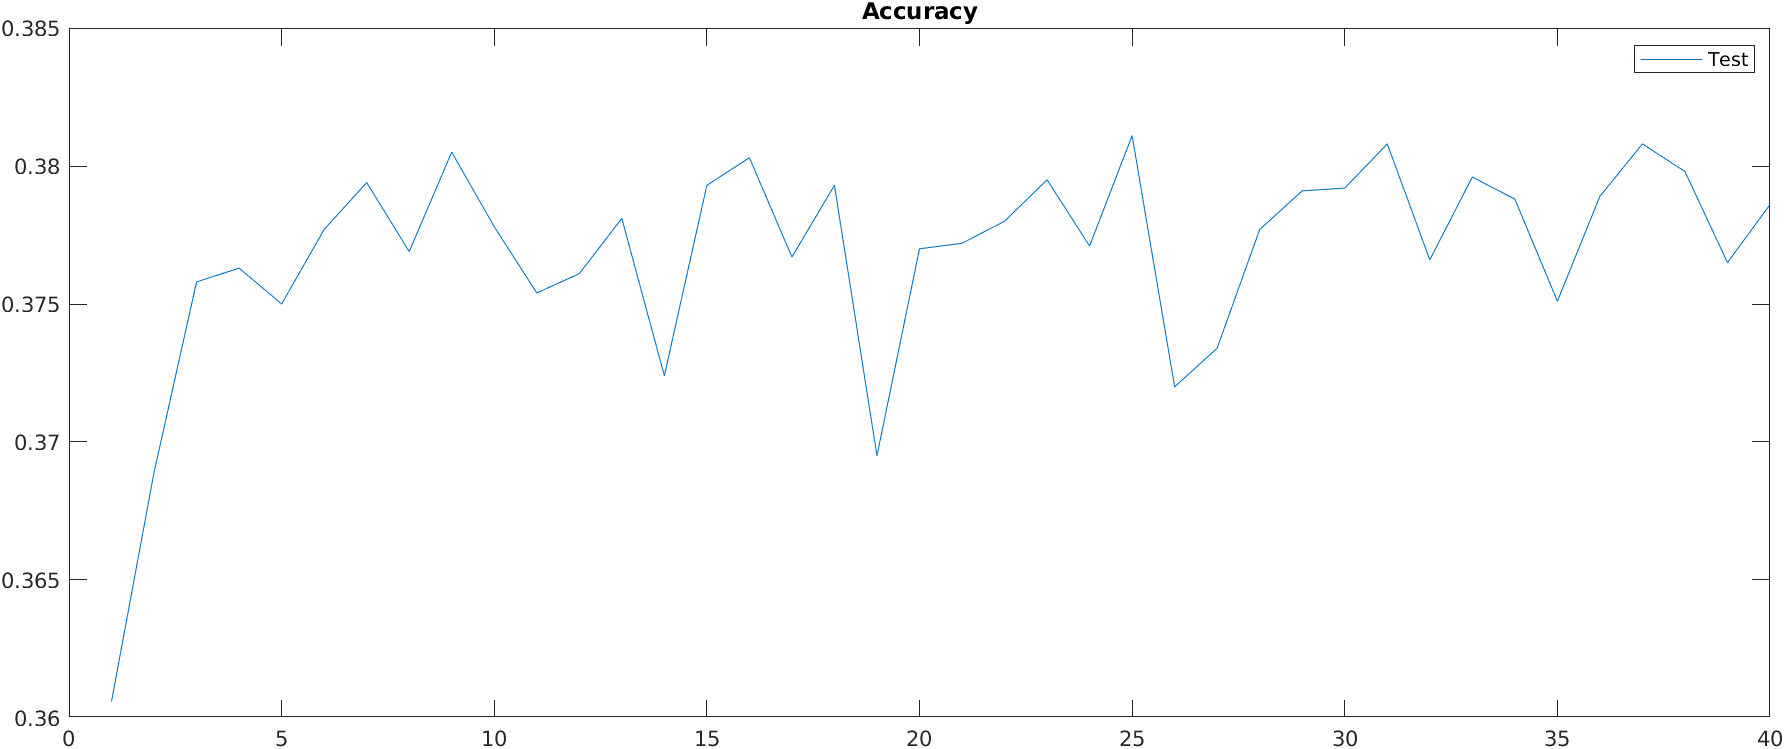
\includegraphics[width=\textwidth]{../code/result_pics/lambda=1, n_epochs=40, n_batch=100, eta=.001 all data for training/accuracy.png}
        \caption{Improvement (i) Accuracy (lambda=1, n\_epochs=40, n\_batch=100, eta=0.001)}
        \label{fig:accuracya}
    \end{figure}
    \begin{figure}[ht]
        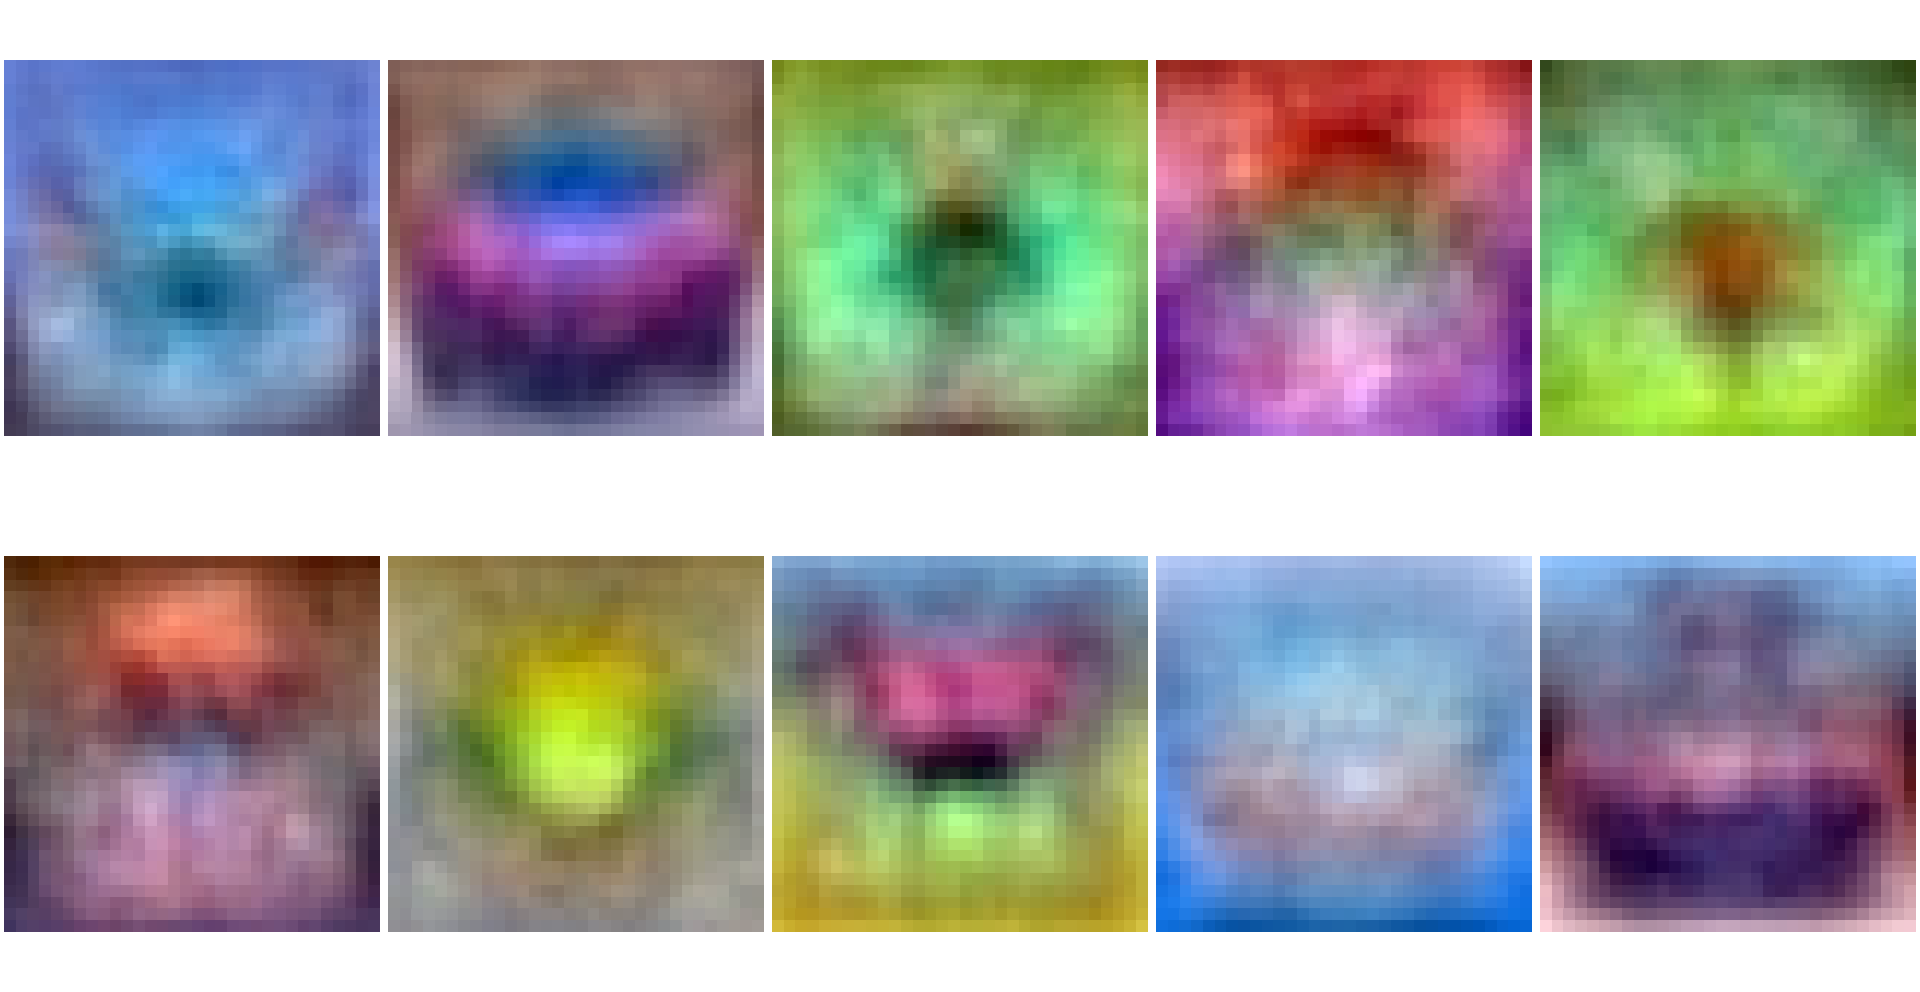
\includegraphics[width=\textwidth]{../code/result_pics/lambda=1, n_epochs=40, n_batch=100, eta=.001 all data for training/weights.png}
        \caption{Improvement (i) Weights (lambda=1, n\_epochs=40, n\_batch=100, eta=0.001)}
        \label{fig:weightsa}
    \end{figure}

\clearpage

\subsection{Results Improvement (ii)}
In this experiment I trained on all available data as in experiment 1 and used the same parameters. I trained the network for 2000 epochs and 
every 100 epochs I stored a snapshot of the diagrams for loss, accuracy and weights. 
Also I logged the values of each epoch to a file (result\_pics/train\_longer/values.csv). After each epoch I compared the training loss to 
the validation loss and set a threshold (0.5) to detect when the network begins to overfit, but in my runs the values stayed very close to each other 
and never exceeded that threshold. The maximum absolute difference over all 2000 epochs was 0.01996.\\
As a result we can observe that training longer does not improve the result that much, but we also see that no overfitting seems to occur. 
We see that during the first 100 epochs the accuracy increases slightly but after that it stays more or less the same.

\begin{table}[ht]
\centering
\begin{tabular}{|l|l|l|l|}
\hline
\textbf{epoch} & \textbf{training loss} & \textbf{validation loss} & \textbf{accuracy} \\ \hline
1              & 2.35312                & 2.36131                  & 36.06\%           \\ \hline
10             & 1.92387                & 1.9376                   & 37.78\%           \\ \hline
50             & 1.92102                & 1.93453                  & 37.55\%           \\ \hline
100            & 1.92044                & 1.93162                  & 37.65\%           \\ \hline
200            & 1.91963                & 1.92828                  & 37.72\%           \\ \hline
300            & 1.92069                & 1.93098                  & 37.64\%           \\ \hline
400            & 1.92159                & 1.93381                  & 37.42\%           \\ \hline
500            & 1.92045                & 1.92874                  & 37.89\%           \\ \hline
600            & 1.9197                 & 1.93142                  & 37.90\%           \\ \hline
700            & 1.91865                & 1.93335                  & 38.25\%           \\ \hline
800            & 1.91992                & 1.93714                  & 38.37\%           \\ \hline
900            & 1.92071                & 1.93663                  & 38.03\%           \\ \hline
1000           & 1.92166                & 1.92969                  & 37.43\%           \\ \hline
\end{tabular}
\caption{Summary of longer training}
\label{tab:summary_longer_training}
\end{table}

    \begin{figure}[ht]
        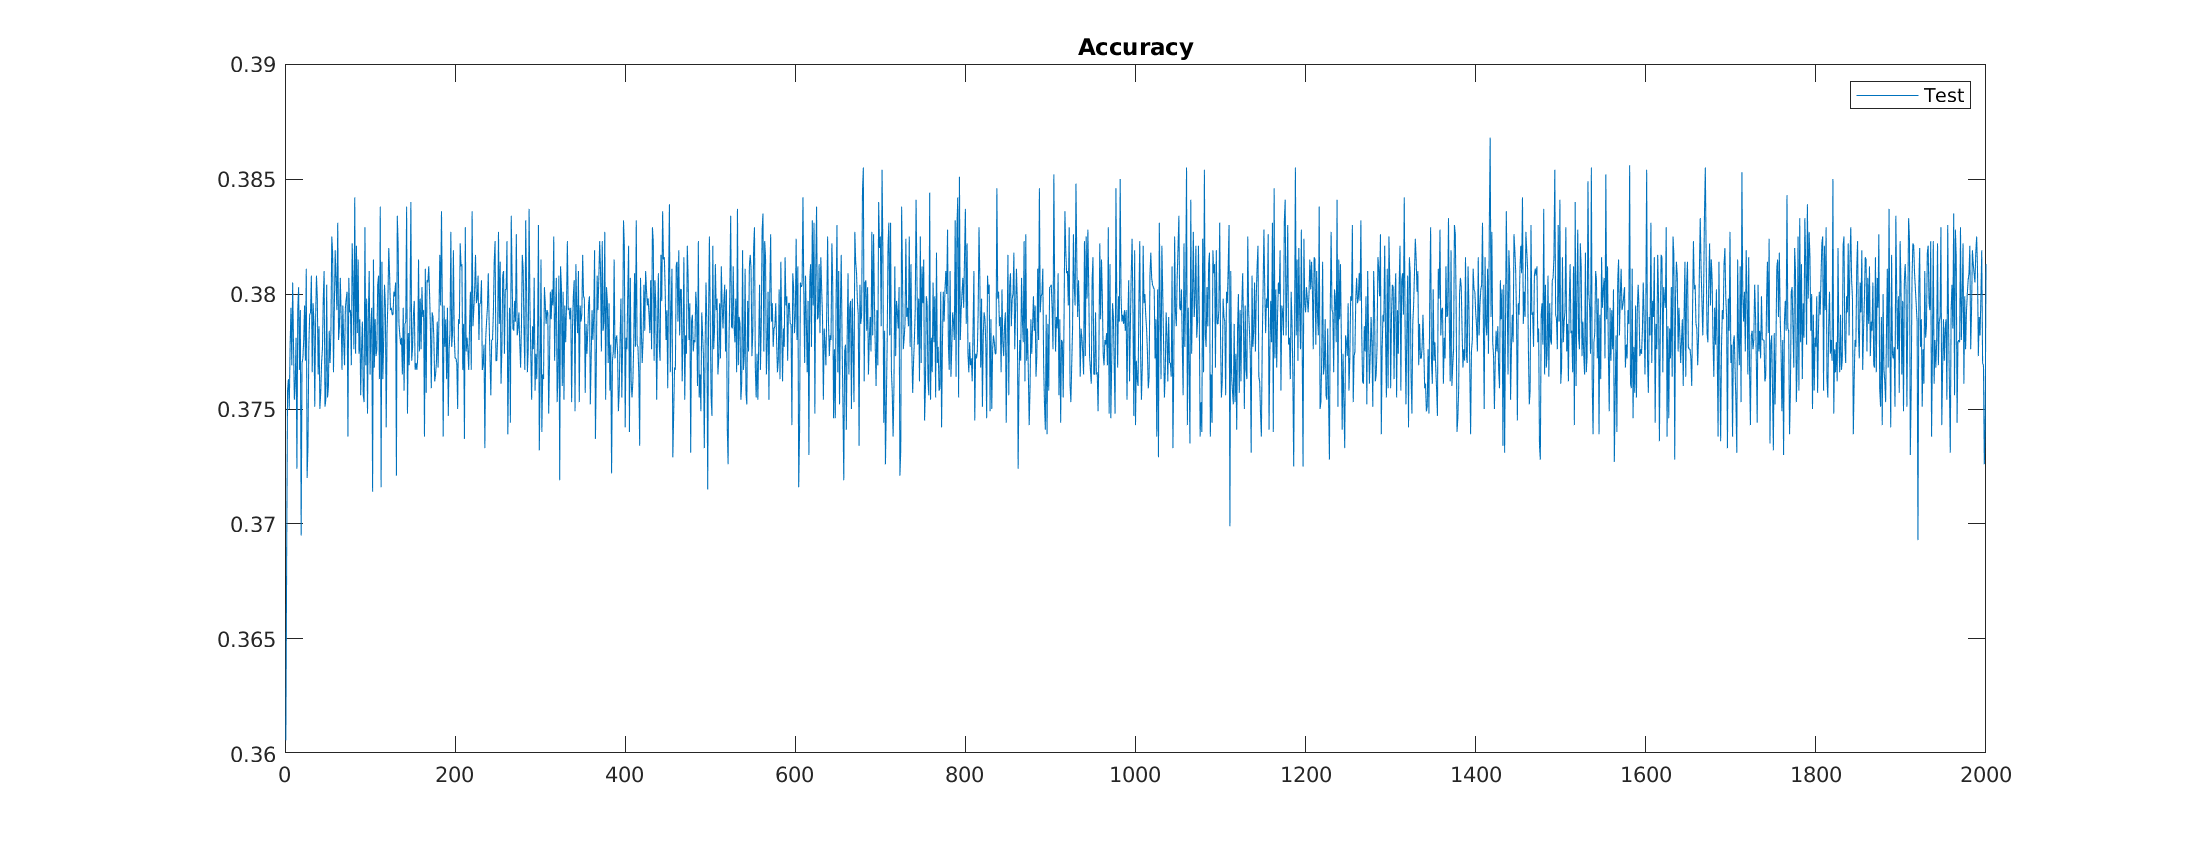
\includegraphics[width=\textwidth]{../code/result_pics/train_longer/2000_accuracy.png}
        \caption{Improvement (ii) accuracy after 2000 epochs}
        \label{fig:accuracyb}
    \end{figure}
    \begin{figure}[ht]
        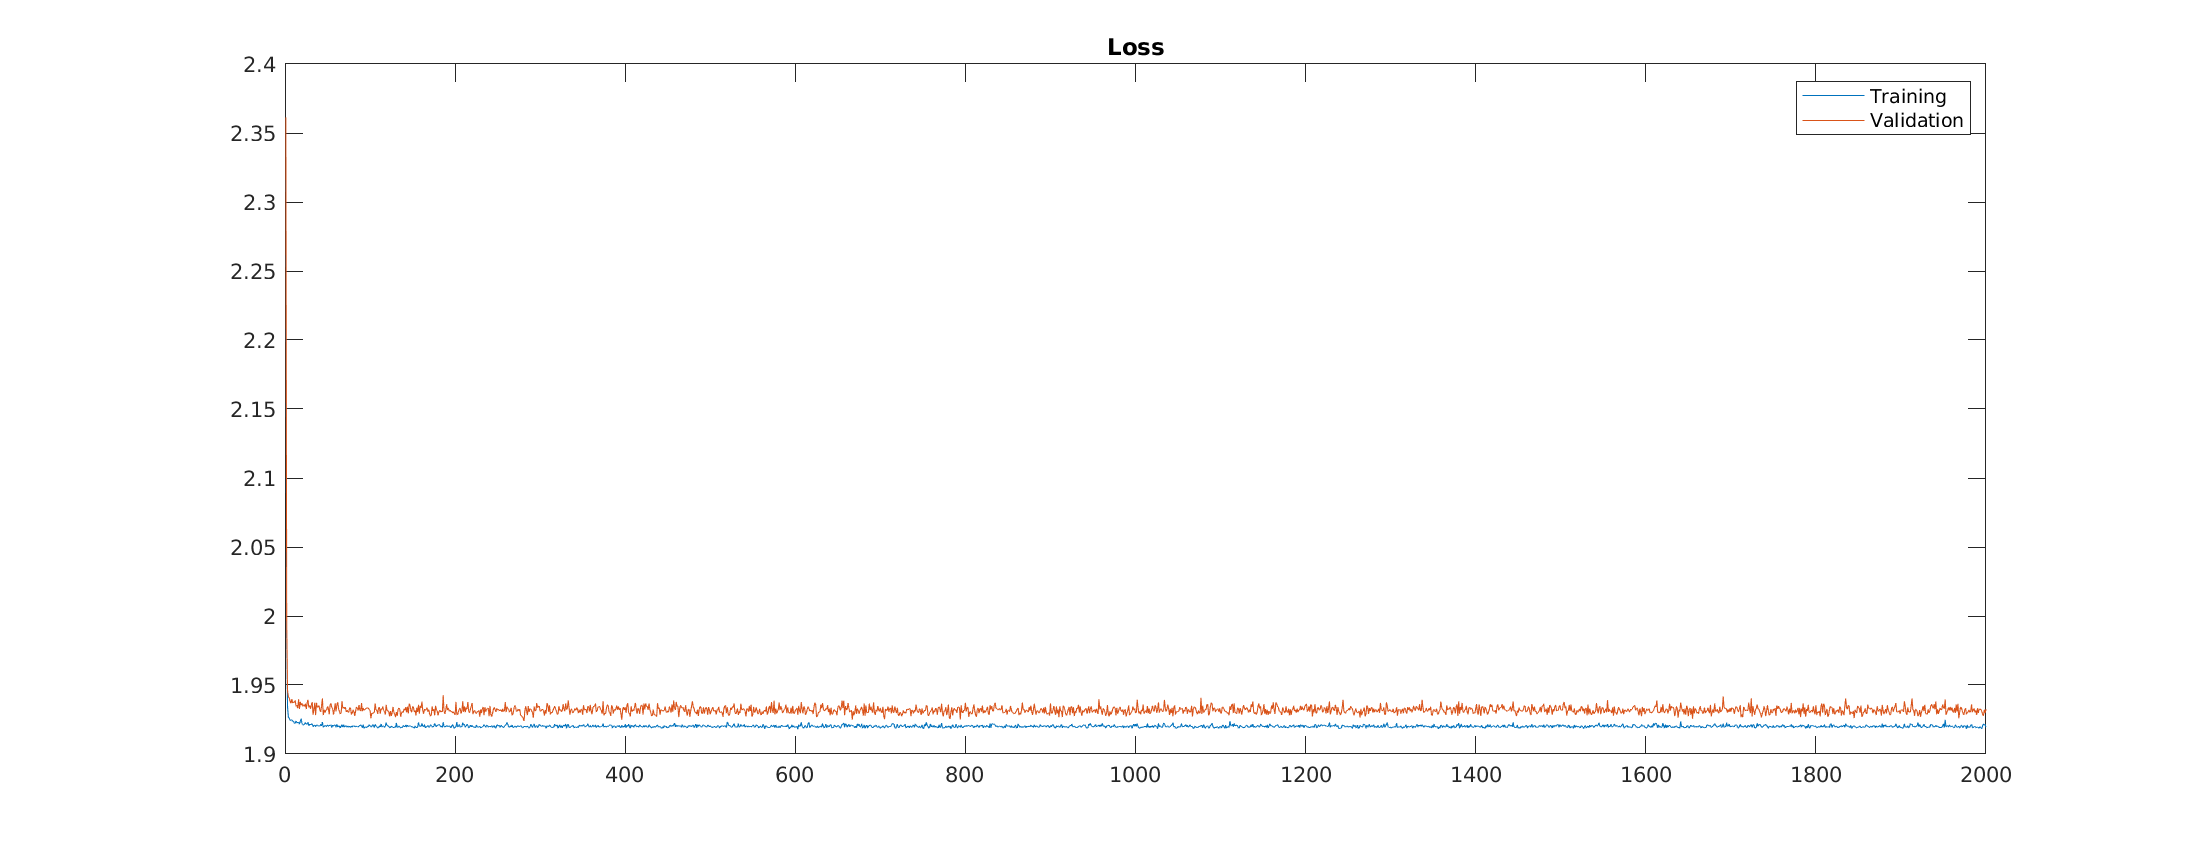
\includegraphics[width=\textwidth]{../code/result_pics/train_longer/2000_loss.png}
        \caption{Improvement (ii) Loss after 2000 epochs}
        \label{fig:lossb}
    \end{figure}
    \begin{figure}[ht]
        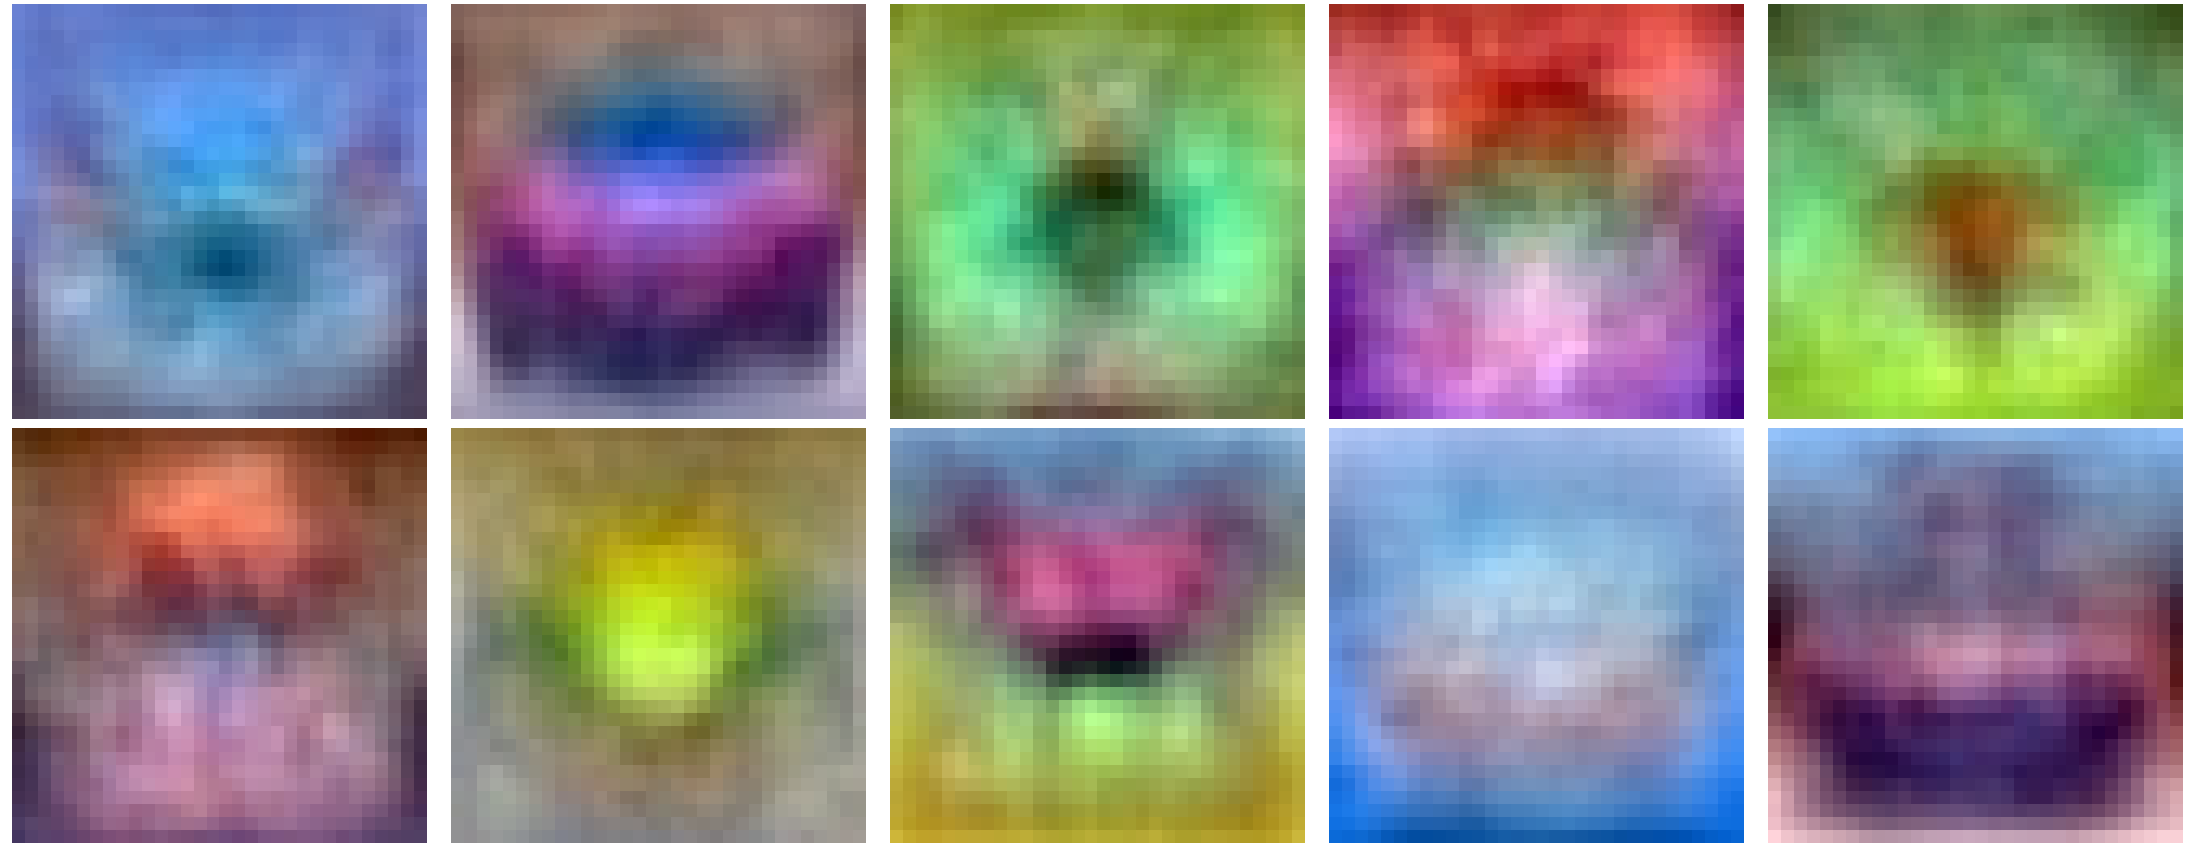
\includegraphics[width=\textwidth]{../code/result_pics/train_longer/2000_weights.png}
        \caption{Improvement (ii) weights after 2000 epochs}
        \label{fig:weightsb}
    \end{figure}

\clearpage

\subsection{Results Improvement (iii)}
All the previous experiments were performed with shuffling the order of the training set. So in this experiment I will not shuffle the order to 
observe if it has a visible effect on the outcome. To switch on shuffling in the training loop I use \(for j=randperm(n/gd\_params.n\_batch)\) and to switch it off I use
\(for j=1:n/gd\_params.n\_batch\).\\
As we can see in the figures below not shuffling the training data results in much smoother accuracy and loss curves.\\
The training results are not very different. Maybe we could conclude that shuffling the training data results in a slightly higher accuracy but the differences are very small.
\begin{table}[ht]
\centering
\begin{tabular}{|l|l|l|l|}
\hline
\textbf{epoch} & \textbf{training loss} & \textbf{validation loss} & \textbf{accuracy} \\ \hline
1              & 2.35301                & 2.35979                  & 35.97\%           \\ \hline
10             & 1.92442                & 1.93682                  & 37.35\%           \\ \hline
50             & 1.92094                & 1.93256                  & 37.52\%           \\ \hline
100            & 1.92058                & 1.93186                  & 37.62\%           \\ \hline
200            & 1.92056                & 1.93169                  & 37.57\%           \\ \hline
300            & 1.92056                & 1.93168                  & 37.58\%           \\ \hline
400            & 1.92056                & 1.93168                  & 37.58\%           \\ \hline
500            & 1.92056                & 1.93168                  & 37.58\%           \\ \hline
\end{tabular}
\caption{Summary - not shuffled}
\label{not_shuffled}
\end{table}

\begin{table}[ht]
\centering
\begin{tabular}{|l|l|l|l|}
\hline
\textbf{epoch} & \textbf{training loss} & \textbf{validation loss} & \textbf{accuracy} \\ \hline
1              & 2.35312                & 2.36131                  & 36.06\%           \\ \hline
10             & 1.92387                & 1.9376                   & 37.78\%           \\ \hline
50             & 1.92102                & 1.93453                  & 37.55\%           \\ \hline
100            & 1.92044                & 1.93162                  & 37.65\%           \\ \hline
200            & 1.91963                & 1.92828                  & 37.72\%           \\ \hline
300            & 1.92069                & 1.93098                  & 37.64\%           \\ \hline
400            & 1.92159                & 1.93381                  & 37.42\%           \\ \hline
500            & 1.92045                & 1.92874                  & 37.89\%           \\ \hline
\end{tabular}
\caption{Summary - shuffled}
\label{shuffled}
\end{table}

\begin{figure}[ht]
    \centering
    \subfloat[\centering shuffle disabled]{{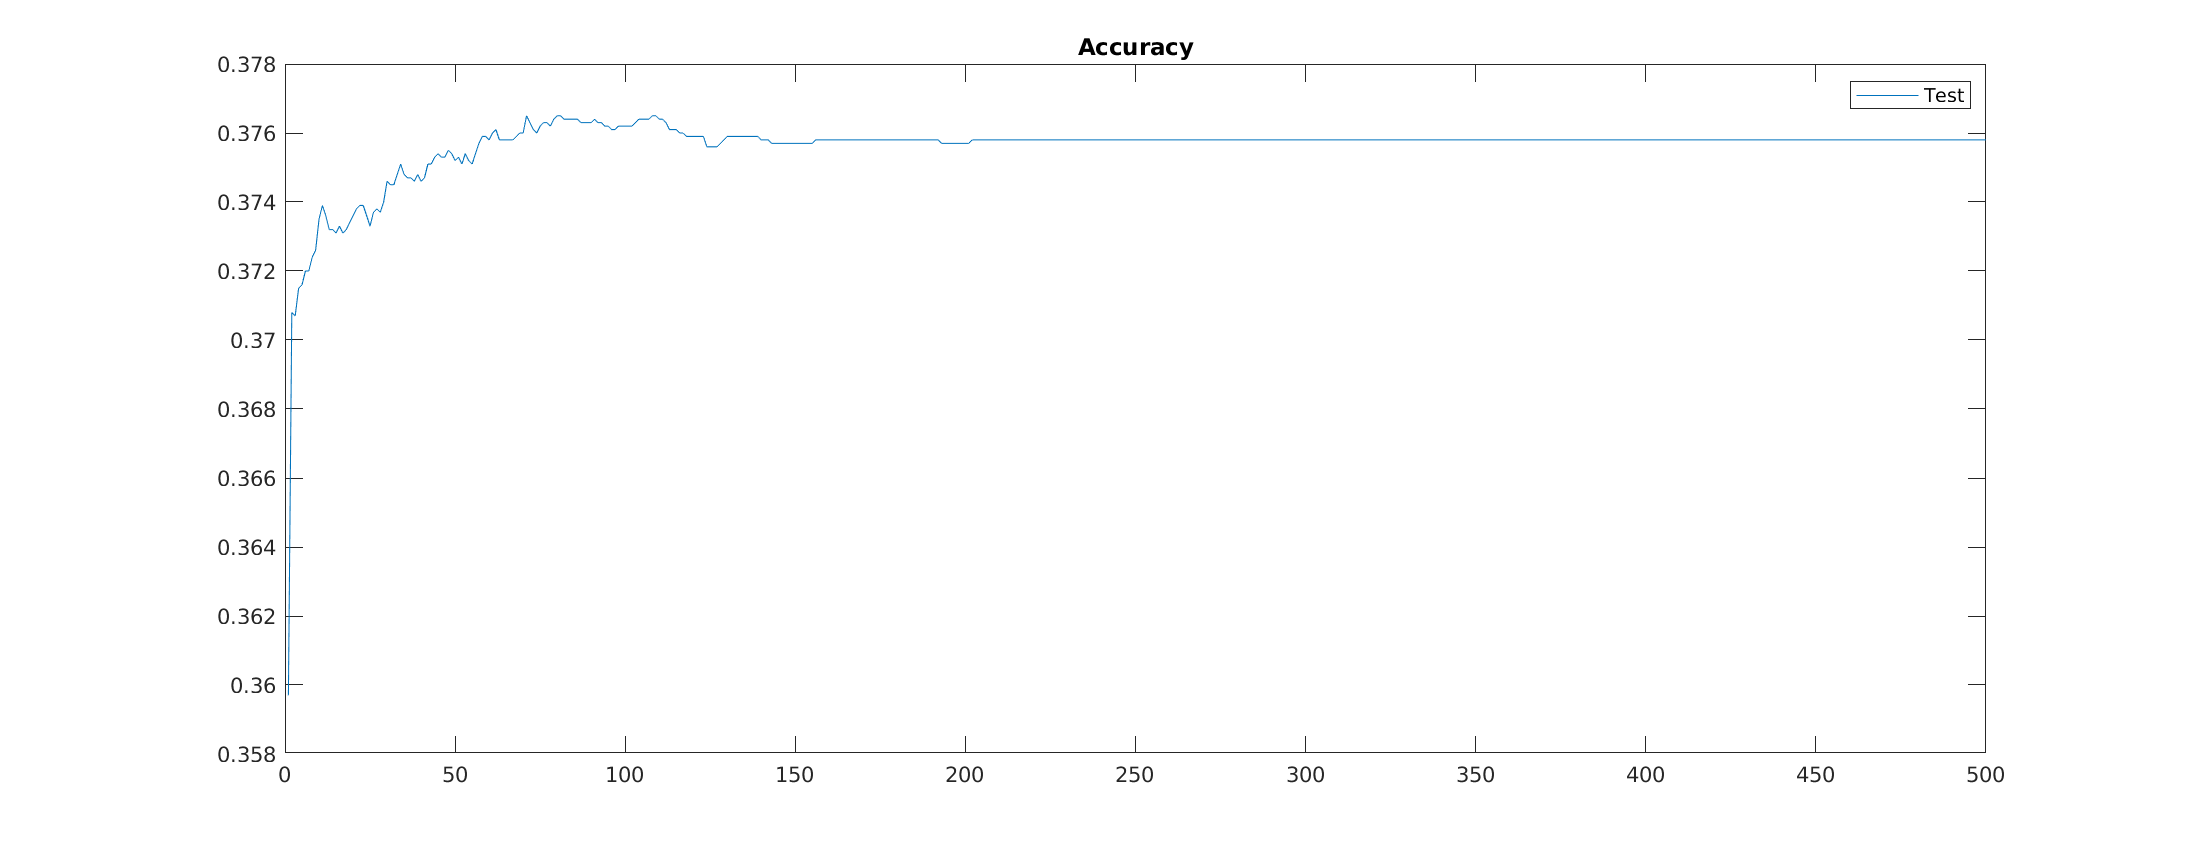
\includegraphics[width=\textwidth]{../code/result_pics/no_shuffling/500_accuracy.png} }}%
    \qquad
    \subfloat[\centering shuffle enabled]{{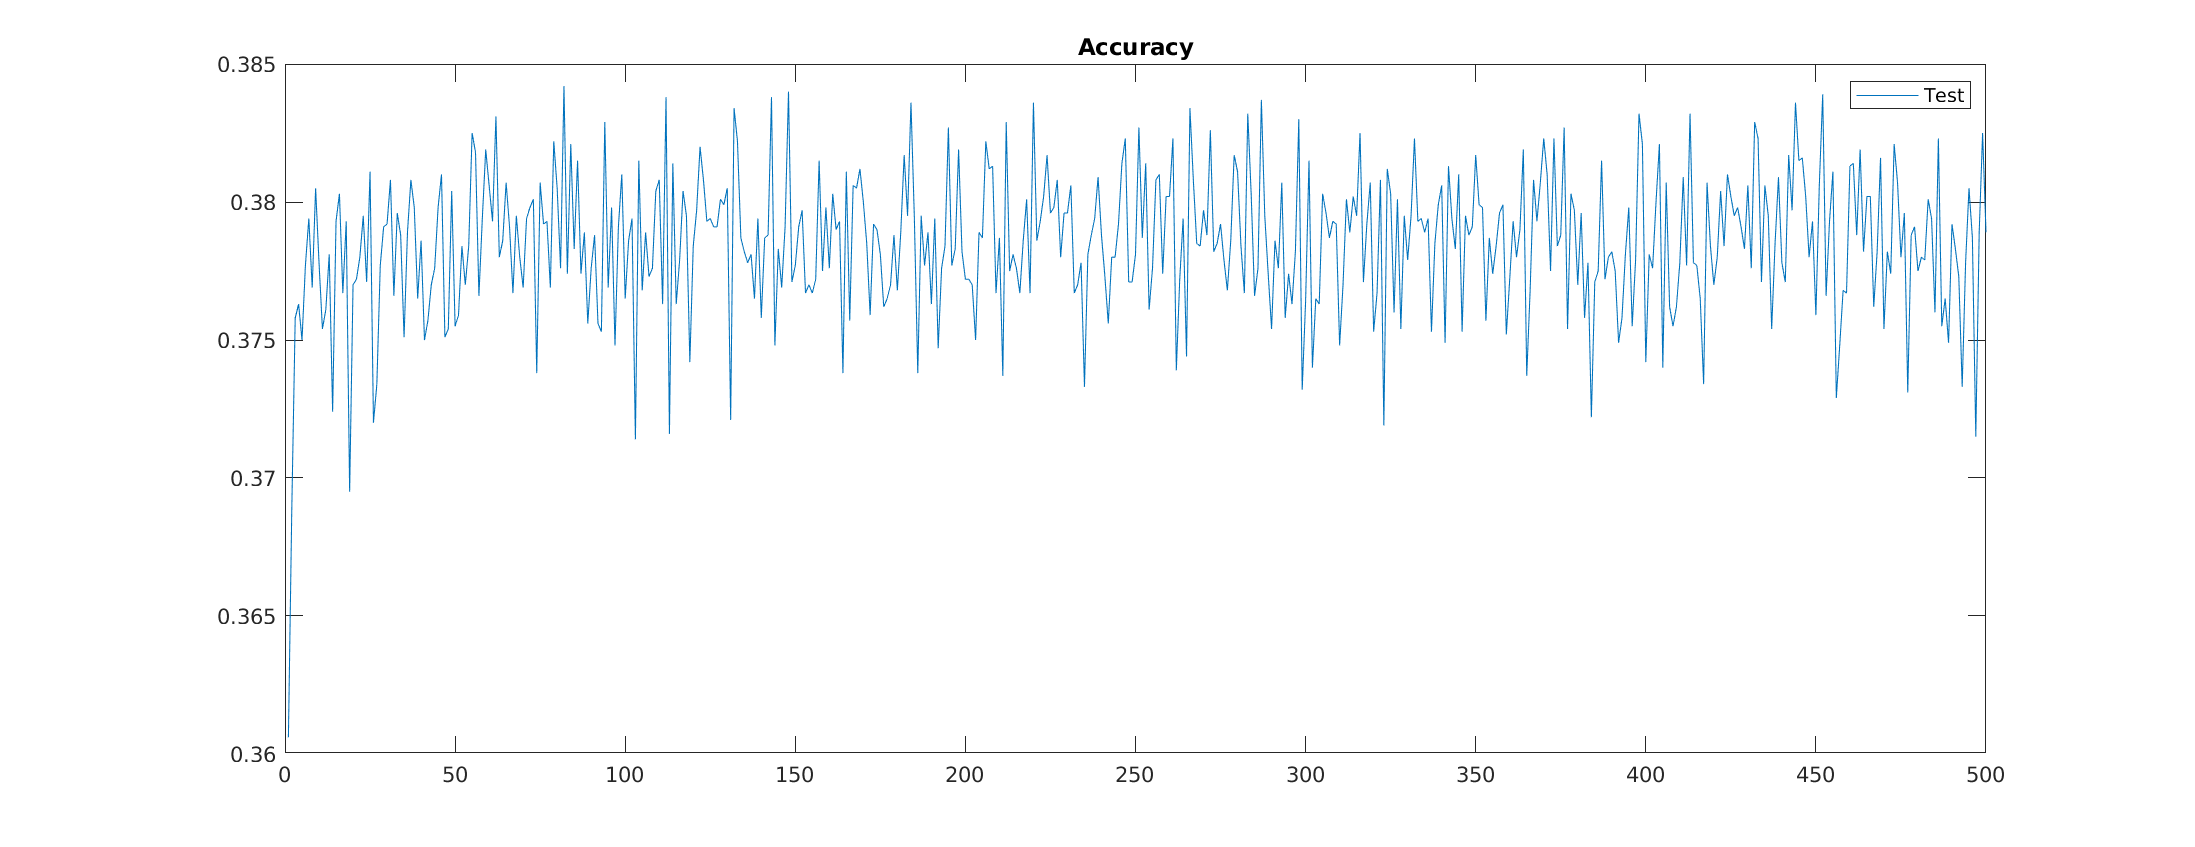
\includegraphics[width=\textwidth]{../code/result_pics/shuffling/500_accuracy.png} }}%
    \caption{Improvement (iii) Accuracy}%
    \label{fig:example}%
\end{figure}
\begin{figure}[ht]
    \centering
    \subfloat[\centering shuffle disabled]{{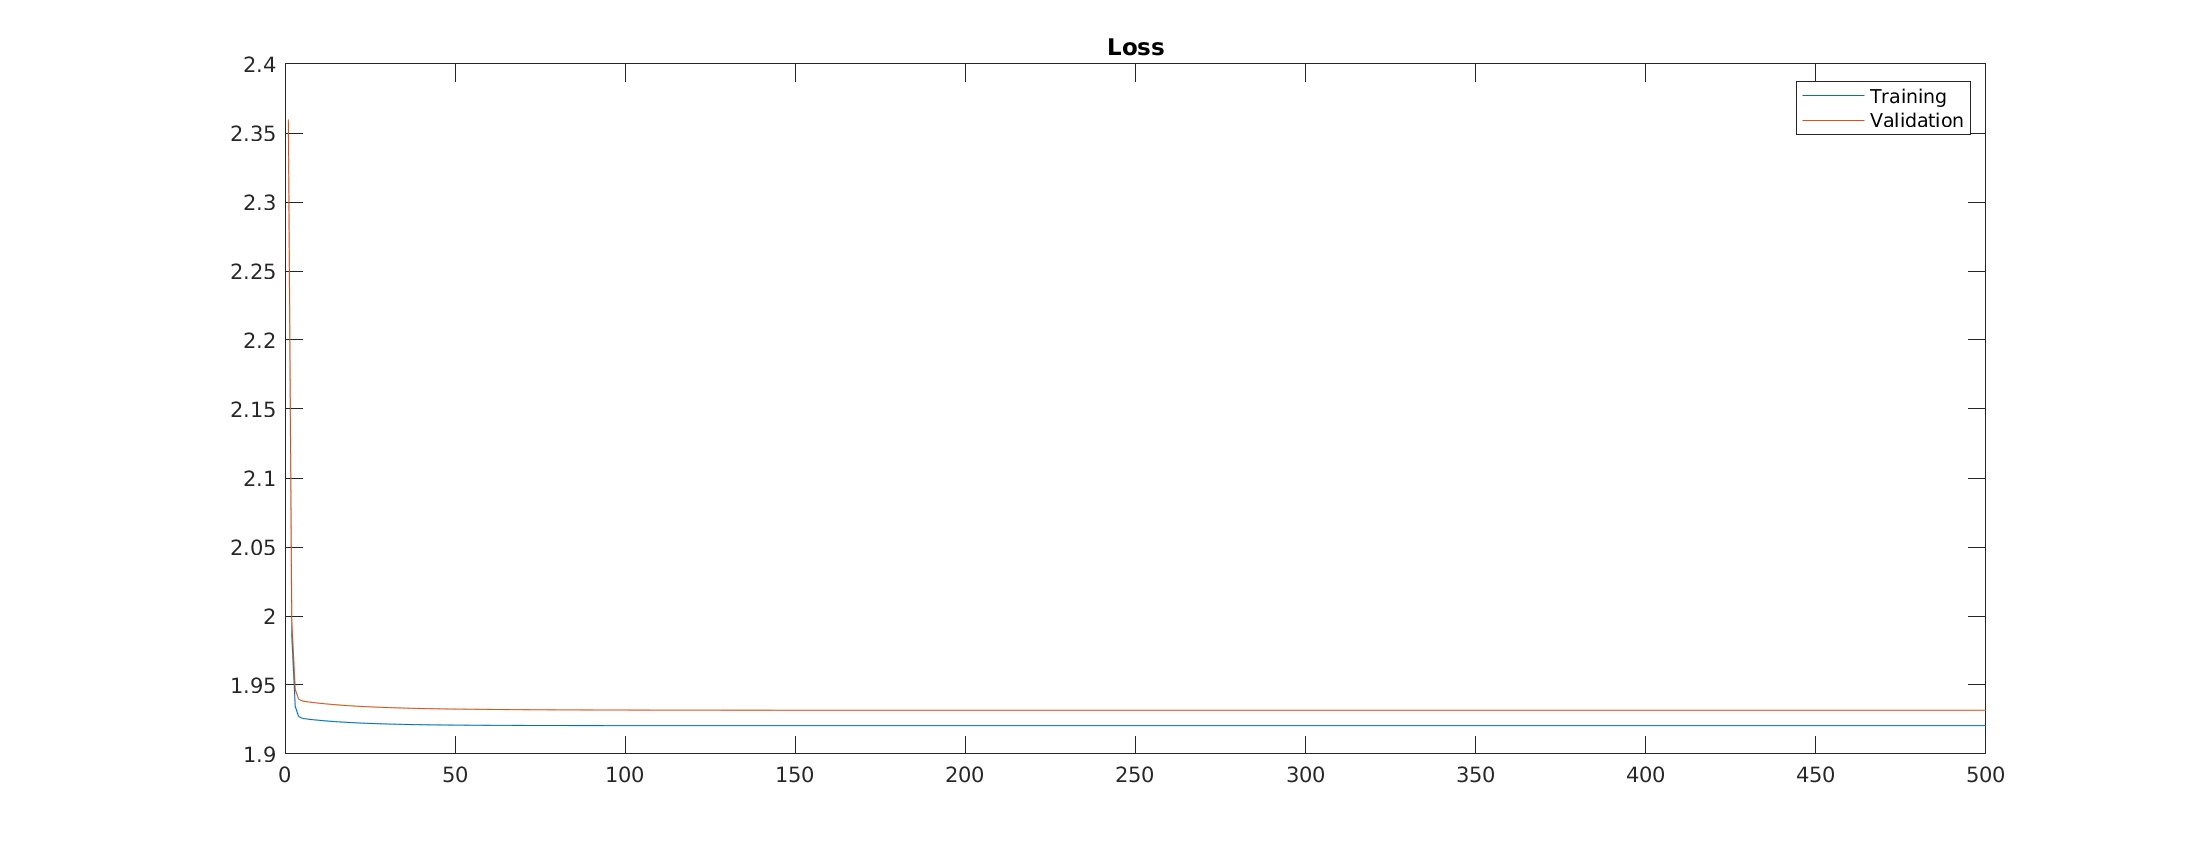
\includegraphics[width=\textwidth]{../code/result_pics/no_shuffling/500_loss.png} }}%
    \qquad
    \subfloat[\centering shuffle enabled]{{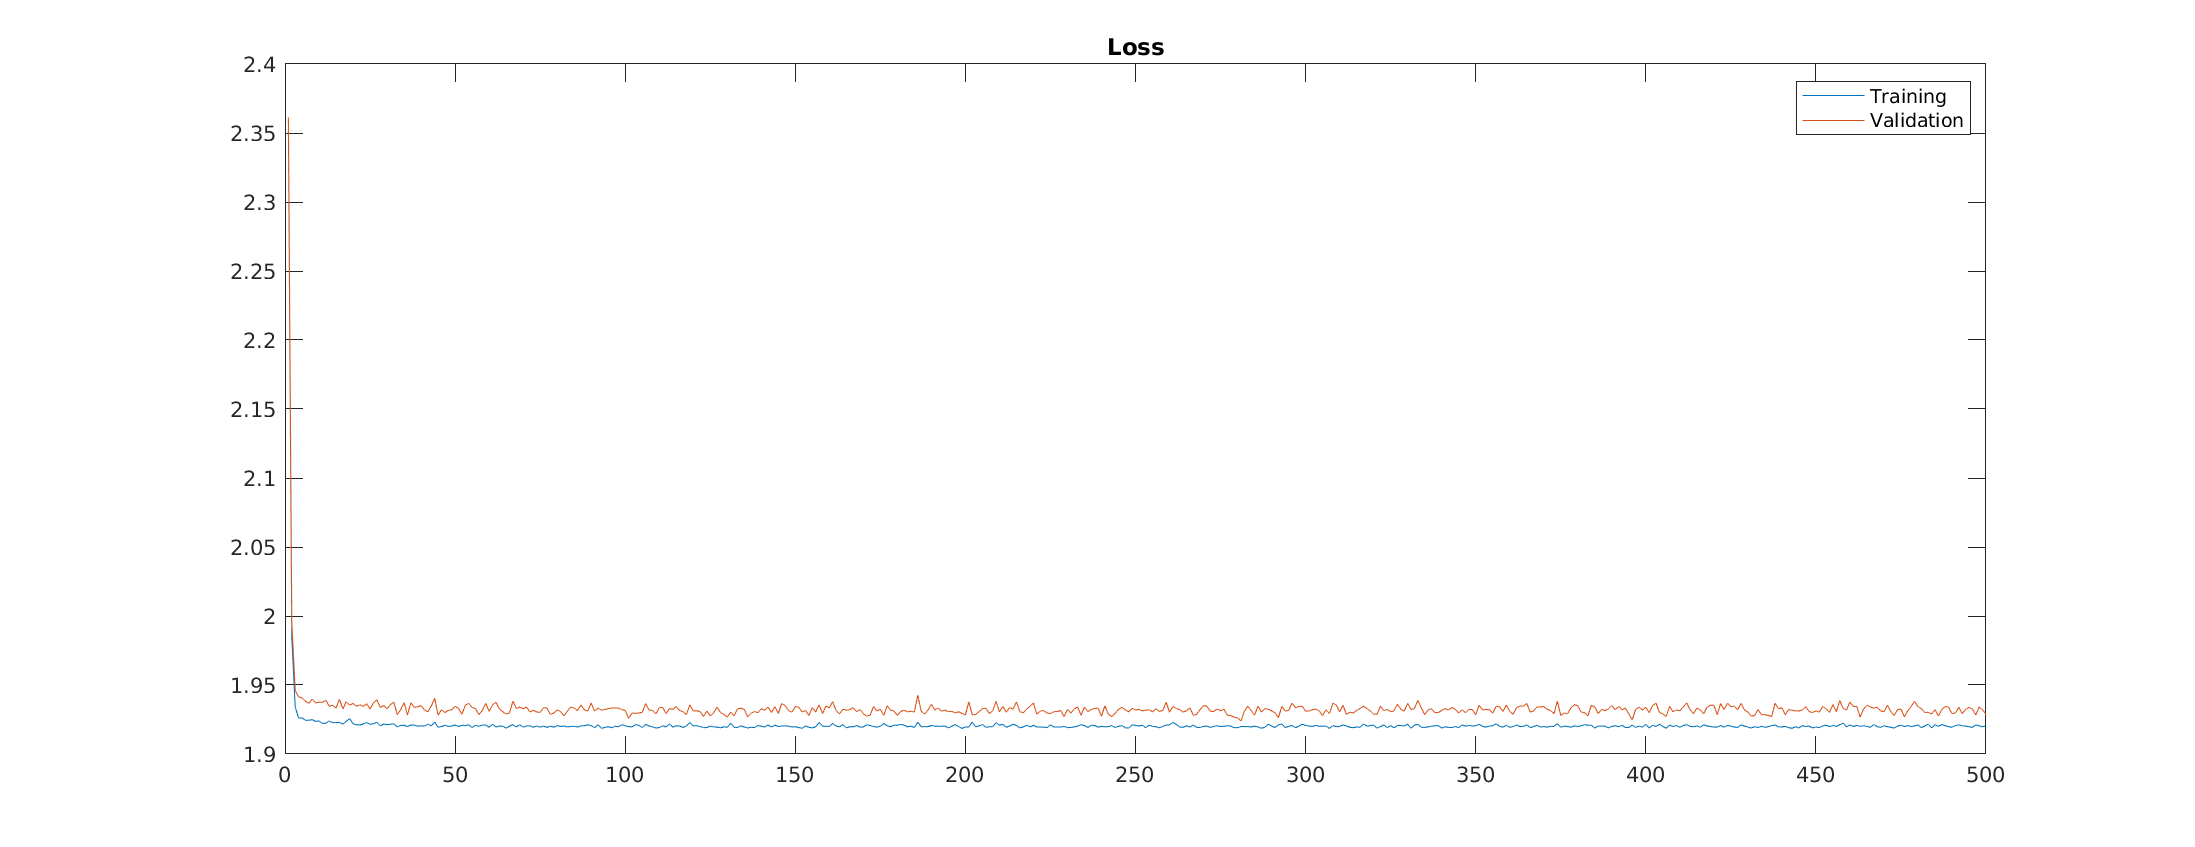
\includegraphics[width=\textwidth]{../code/result_pics/shuffling/500_loss.png} }}%
    \caption{Improvement (iii) Loss}%
    \label{fig:example}%
\end{figure}
\begin{figure}[ht]
    \centering
    \subfloat[\centering shuffle disabled]{{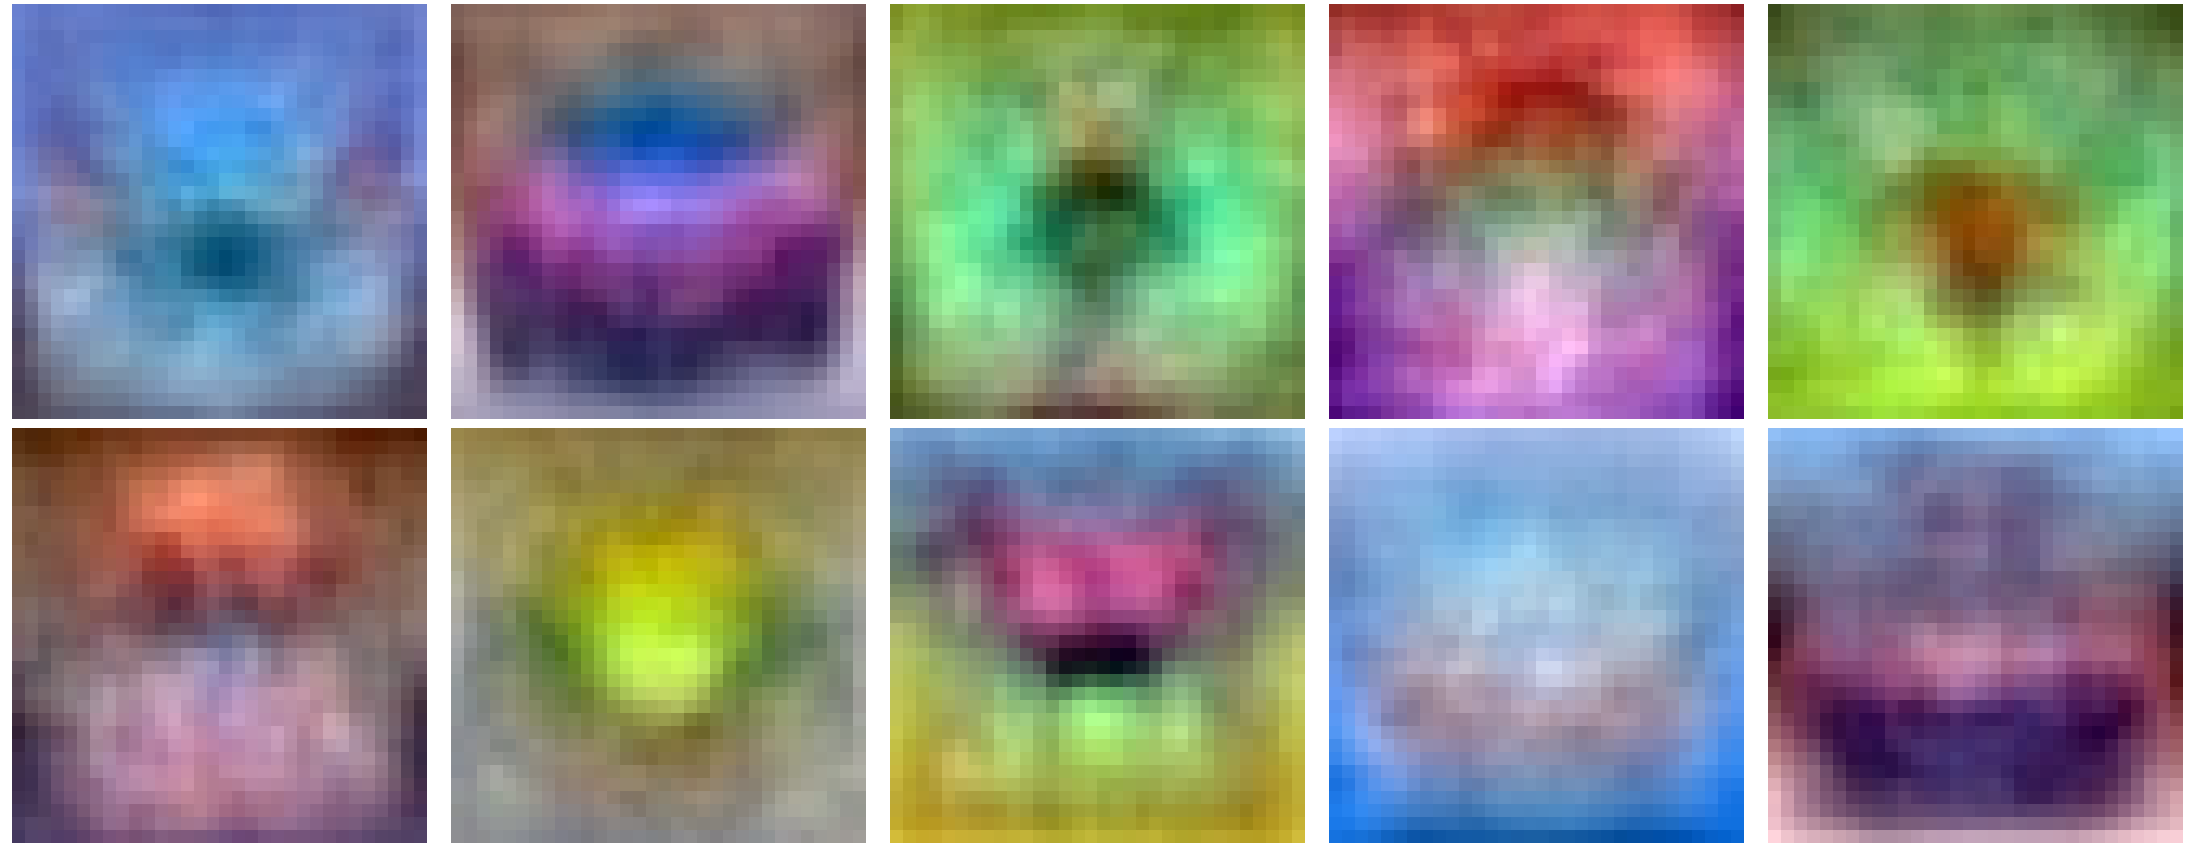
\includegraphics[width=\textwidth]{../code/result_pics/no_shuffling/500_weights.png} }}%
    \qquad
    \subfloat[\centering shuffle enabled]{{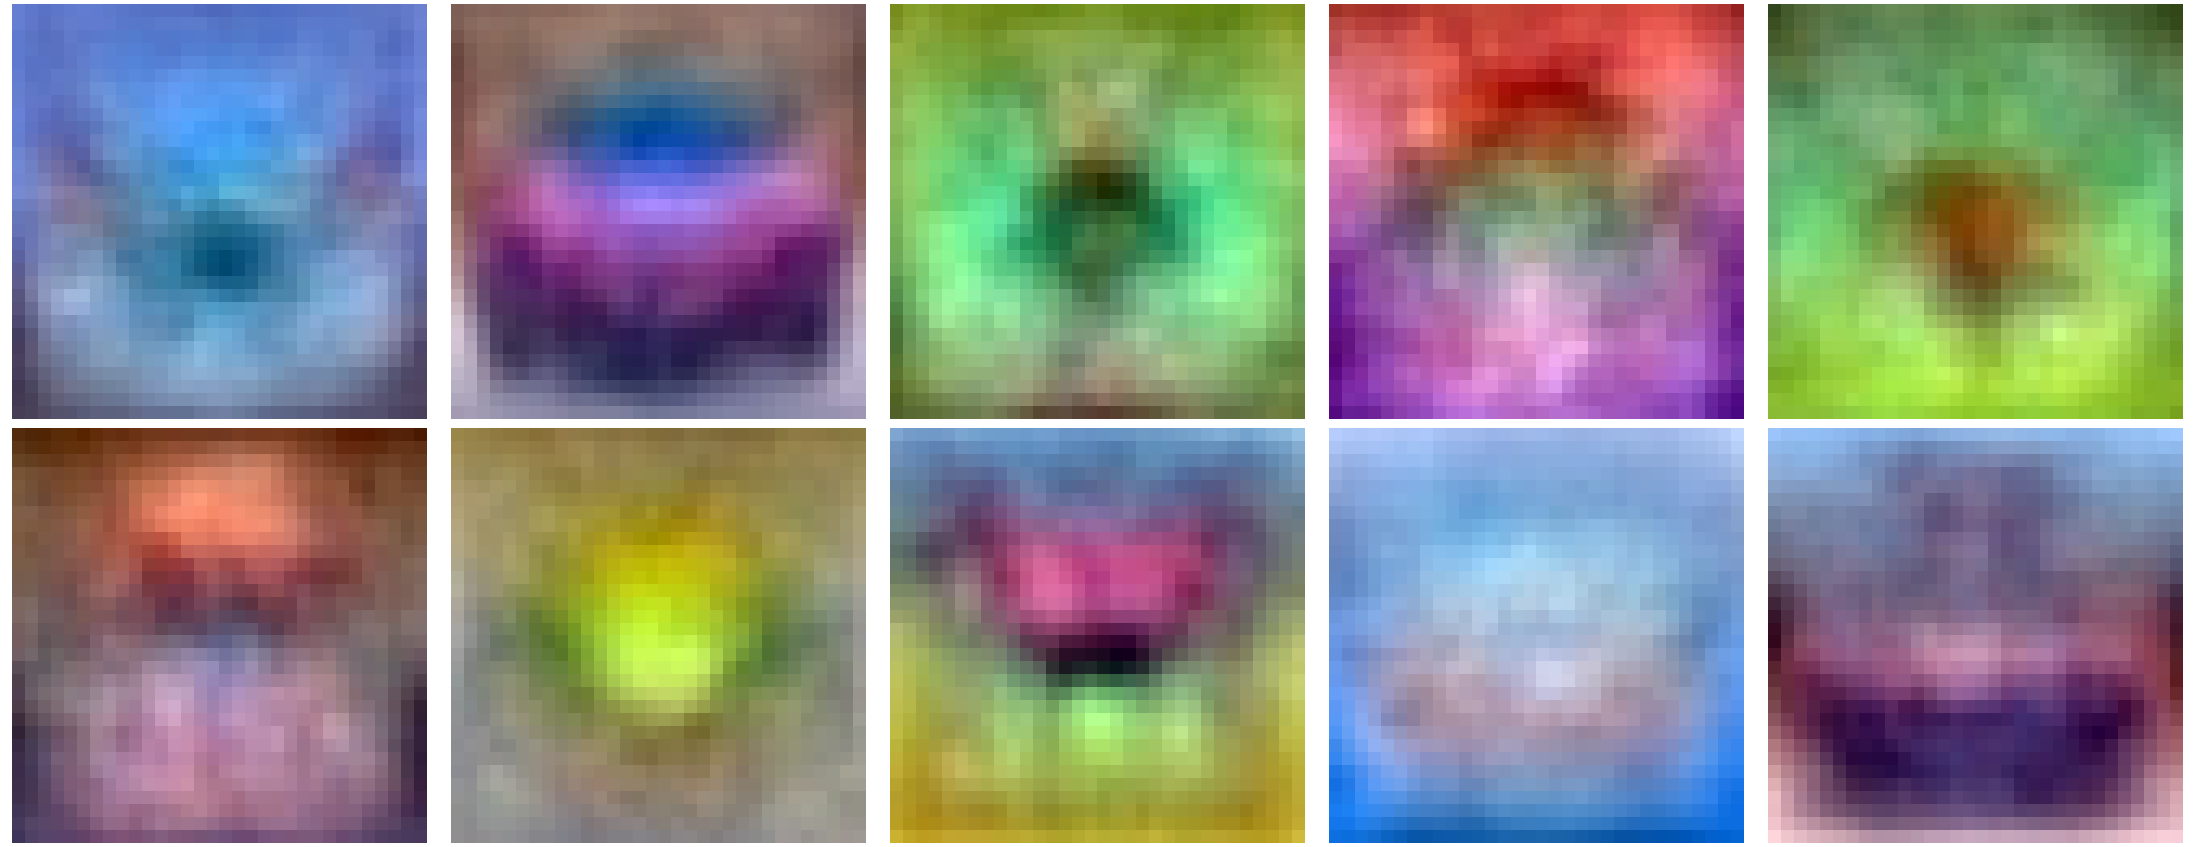
\includegraphics[width=\textwidth]{../code/result_pics/shuffling/500_weights.png} }}%
    \caption{Improvement (iii) Weights}%
    \label{fig:example}%
\end{figure}